\label{chpt:introduction}

Achieving the one exaFLOP performance necessary from an exascale computer will
require modifications to current hardware architecture which will in turn affect
the design of programming models and their runtime
systems~\cite{article-kogge}.  Until recent years, performance increased in
keeping with \emph{Moore's Law}: the number of transistors within an integrated
circuit doubled approximately every two years.  As we reached a limit on the
number of transistors a single chip could contain, hardware architects had to
look for other ways to keep up with performance advancement expectations. In
most cases, this involved a greater emphasis on parallelism. Consequently, in
order to take advantage of hardware advances, applications, runtimes, and
programming models have often required redesign, if not reimplementation.

As we look towards the next generation of high-performance computing
(HPC) systems, a shift in application design is again anticipated,
this time to reach exascale performance. On-chip parallelism along
with reduced data movement will be critical for applications to make
optimal use of the hardware and minimize power consumption.

Conventional language semantics will not be sufficient
to exploit the architectural advances being developed such as
inter-core message queues. Therefore, new parallel programming models
and smarter runtime systems are being developed to support
them~\cite{article-gottlieb}.  The majority of these models are
\emph{data-centric} rather than \emph{compute-centric}: they allow, for
instance, the runtime scheduler to prioritize scheduling computation on nodes
or cores where the required information already resides rather than the next
available processor~\cite{article-kogge}. This kind of model reduces
communication, the predicted bottle neck for exascale systems.

The information produced as output from HPC applications such as fluid
simulations or finite-element models tends to scale in size with
compute power. This is expected to occur with exascale systems as well
and has produced a need for visualization algorithms that can take
advantage of distributed systems as well as an opportunity to design
algorithms that can be integrated into HPC applications to produce
results during execution~\cite{proceedings-brownlee}.  Chapter~\ref{chpt:design}
proposes one such design for ray tracing, a commonly used rendering technique.

The rest of this thesis is organized as follows: we start with a description of
exascale along with a description of the projected trends in programming models
that will perform well on exascale.  We then explore one programming model,
CnC, that is expected to map well to exascale systems.  After describing the
CnC programming model we analyze current ray tracing algorithms and propose
places for improvement for exascale.  Specifically, we look at ways we can
reduce communication overhead within the algorithm.  We then describe the
implementation of a ray tracer developed using \emph{Concurrent Collections},
Intel's CnC implementation.  Chapter~\ref{chpt:implementation} describes the
implementation of the designed algorithm and Chapter~\ref{chpt:evaluation}
evaluates how it performs on today's architecture as well as speculates as to
how it might perform on future exascale hardware.  Finally we conclude with a
chapter on future work.

\section{Exascale}
\label{sec:exascale}

Until 2004, performance of single-core microprocessors increased as
predicted as a result of smaller and faster transistors being
developed (i.e. Moore's Law). At that time, this trend shifted as we
reached an inflection point caused by a chips power dissipation
~\cite{article-kogge}. Unable to sufficiently and inexpensively
cool a chip, chip designers looked for other ways to increase
performance. This came in the form of multi-core processors, which are
now the building blocks of many HPC (and other) systems.

The introduction of multi-core processors on each node of a cluster
caused a shift in parallel application design. Programs using the
cross-platform standard Message Passing Interface (MPI) library
~\cite{book-snir} could not efficiently exploit parallelism
on individual nodes without a rewrite of the underlying algorithms.
The Open Multi-Processing (OpenMP) ~\cite{openmp08} library presented
a cross-platform standard for parallel programming on multicore nodes,
which led to the emergence of hybrid systems that mixed MPI and
OpenMP. The cluster would run a collection of MPI processes, one per
node, and each node would then execute an OpenMP program redesigned
from the original single-threaded program which used a fixed number of
threads to execute a single work-sharing construct, such as a parallel
loop ~\cite{article-gropp}.

Although the exact form of an exascale ecosystem is unknown, research
suggests that data movement will overtake computation as the dominant
cost in the system~\cite{article-kogge}.  This results from the primary
means of increasing parallelism on future systems as being on-chip.  Some
predictions suggesting hundreds or even thousands of cores per chip die.
As a result, we will would see a higher available bandwidth on
chip along with lower latencies for communication within a node. The
lower overhead within a chip would therefore provide a significant incentive to
develop \emph{communication avoiding} algorithms.

Two means to avoid communication are, first, to re-compute values
instead of communicating results when possible and, second, to take
account of the need to minimize communication when partitioning the
algorithm into parallel functional units.

Many of our current programming models lack the semantics necessary to
implement communication-avoiding algorithms. As a result, new
languages with additional semantics are being proposed for exascale
systems. A common theme among these languages is the ability to
statically declare dependencies and locality information.  These additional
details can then be used by the runtime to aid in scheduling and anticipatory
data movement.

\section{Ray Tracing}
\label{sec:raytracing}

Ray tracing is one of the rendering techniques often used in computer graphics 
to render three-dimensional scenes into two dimensional
images~\cite{book-shirley}.  A ray tracing renderer takes a set of
objects in 3D space as input and then casts viewing rays into the scene to
determine the color of each pixel in an output image.  

As outlined in Shirley~\cite{book-shirley}, ray tracing has
three main components, ray generation, ray intersection and shading.  The first
component is responsible for computing viewing rays, which are rays from an
origin position to a point on an image plane.  An image plane is the plane that
will contain the final output image.  Conceptually, it is positioned between the
eye, or origin, and the scene to be rendered.  The image plane is highlighted in
Figure~\ref{fig:image-plane}.

\begin{figure}[!htb]
  \centering
  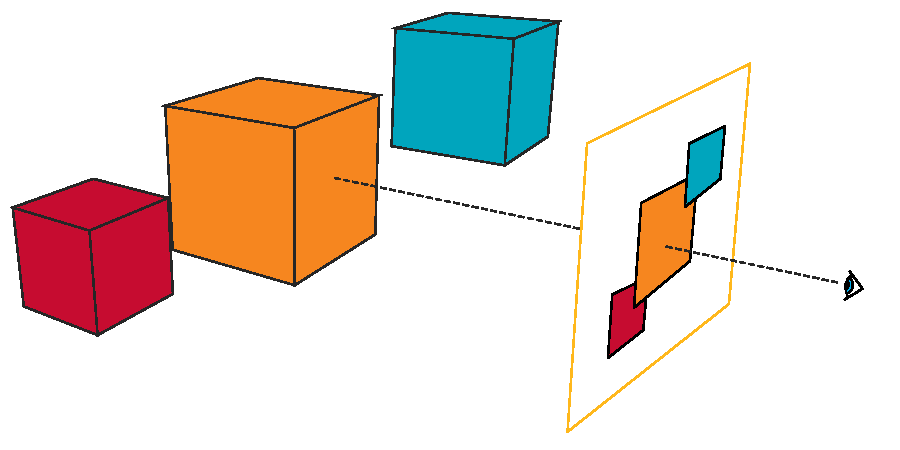
\includegraphics[width=\textwidth]{drawings/examples/cubes_visio_ray_tracing.pdf}
  \caption{Example - Ray Tracing Image Plane}
  \label{fig:image-plane}
\end{figure}

Each viewing ray is then cast into the scene where we apply the second component, 
ray intersection.  For each ray we need to know what object in the scene it 
intersects first.  This tells us which object can be seen by that viewing ray,
allowing us to color the pixel of the image that the viewing ray passed through
by shading, the third component, our intersected object.  Most shading models 
require information from a second set of rays in order to compute the correct 
color.  This second set of rays, or secondary rays, include light rays,
reflected rays and refracted rays.
